\documentclass[tikz,border=5mm]{standalone}
\usepackage{fontawesome5}
\usetikzlibrary{positioning, fit, backgrounds, arrows.meta, calc}

\begin{document}
\begin{tikzpicture}[
    box/.style={
        rectangle,
        rounded corners=3mm,
        draw=black,
        thick,
        fill=pink!20,
        align=center,
        inner sep=3mm
    },
    arrow/.style={
        -Stealth,
        thick
    },
    % Estilos para las copias de vídeo con transparencia y efecto "atrás"
    video-back3/.style={
        opacity=0.35, % Mayor transparencia para las más lejanas
        inner sep=0pt
    },
    video-back2/.style={
        opacity=0.55,
        inner sep=0pt
    },
    video-back1/.style={
        opacity=0.75,
        inner sep=0pt
    },
    video-front/.style={
        opacity=1.0, % Totalmente opaco para la principal
        inner sep=0pt
    }
]

% --- Nodos Principales ---

% Copia 3
% \node[video-back3] (img_back3) at (0.45, 0.3) {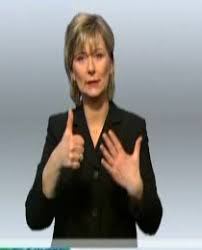
\includegraphics[width=2.2cm]{phoenix.jpg}};
% % Copia 2
% \node[video-back2] (img_back2) at (0.3, 0.2) {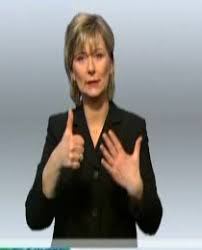
\includegraphics[width=2.2cm]{phoenix.jpg}};
% % Copia 1
% \node[video-back1] (img_back1) at (0.15, 0.1) {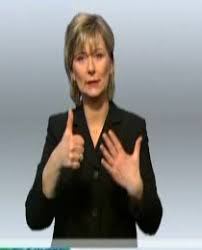
\includegraphics[width=2.2cm]{phoenix.jpg}};
% Imagen Frontal (Principal, opaca)
% Definimos la posición central (0,0) para esta, y las anteriores son relativas
\node[video-front] (img_front) at (0, 0) {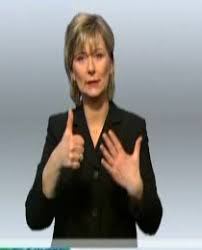
\includegraphics[width=2.2cm]{phoenix.jpg}};

% Nodo Modelo End-to-End (E2E)
\node[box, minimum width=4cm, minimum height=1.8cm] (e2e) at (5, 0) {};
\node[inner sep=0pt] (e2e-icon) at (4.0, 0) {\Large\faCogs};
\node[font=\bfseries\sffamily, right=0.15cm of e2e-icon] {\textit{End-to-end}};

% Nodo Texto Final
\node[box, minimum width=4.5cm, minimum height=1.8cm, text width=4.2cm, align=center] (text) at (12, 0) {\textbf{\sffamily ``Hoy hace calor\\	en sevilla''}};

% --- Conexiones (Flechas Directas Horizontales) ---
% Imagen a Modelo E2E
\draw[arrow] (img_front.east) -- (e2e.west);

% Modelo E2E a Texto (Con etiqueta TEXTO)
\draw[arrow] (e2e.east) -- node[fill=blue!10, inner sep=2pt, font=\small\sffamily\bfseries] {TEXTO} (text.west);

% --- Recuadro de Fondo (Gigante Azul) ---
\begin{scope}[on background layer]
    \node[draw=blue!60, fill=blue!10, thick, rounded corners=1cm,
          % Incluimos la imagen más retrasada y la más adelantada en el fit
          fit=(img_front) (e2e) (text),
          inner xsep=0.8cm, inner ysep=0.8cm] {};
\end{scope}

\end{tikzpicture}
\end{document}
